\documentclass{article}


% if you need to pass options to natbib, use, e.g.:
%     \PassOptionsToPackage{numbers, compress}{natbib}
% before loading neurips_2022


% ready for submission
%\usepackage{neurips_2022}
\usepackage[preprint]{neurips_2022}
\usepackage{amsmath}
\usepackage{amsthm}
\usepackage{amssymb}
\usepackage{color}
\usepackage{graphicx}
\usepackage{subcaption}
\usepackage{booktabs}


% to compile a preprint version, e.g., for submission to arXiv, add add the
% [preprint] option:
%     \usepackage[preprint]{neurips_2022}


% to compile a camera-ready version, add the [final] option, e.g.:
%     \usepackage[final]{neurips_2022}


% to avoid loading the natbib package, add option nonatbib:
%    \usepackage[nonatbib]{neurips_2022}


\usepackage[utf8]{inputenc} % allow utf-8 input
\usepackage[T1]{fontenc}    % use 8-bit T1 fonts
\usepackage{hyperref}       % hyperlinks
\usepackage{url}            % simple URL typesetting
\usepackage{booktabs}       % professional-quality tables
\usepackage{amsfonts}       % blackboard math symbols
\usepackage{nicefrac}       % compact symbols for 1/2, etc.
\usepackage{microtype}      % microtypography
\usepackage{xcolor}         % colors

\newcommand{\pouriacomment}[1]{\textcolor{darkgreen}{[#1]$_{\rm Pouria}$}}
\newcommand{\fgibou}[1]{\textcolor{blue}{[#1]$_{\rm FG}$}}

\title{Neuro-symbolic hybridization of finite discretization methods for solving partial differential equations}


% The \author macro works with any number of authors. There are two commands
% used to separate the names and addresses of multiple authors: \And and \AND.
%
% Using \And between authors leaves it to LaTeX to determine where to break the
% lines. Using \AND forces a line break at that point. So, if LaTeX puts 3 of 4
% authors names on the first line, and the last on the second line, try using
% \AND instead of \And before the third author name.


\author{
  Pouria A. Mistani$^\dagger$\thanks{corresponding author.} \\
  NVIDIA\\
  Santa Clara, CA 95051 \\
  \texttt{pmistani@nvidia.com} \\
  % examples of more authors
  \And
  Samira Pakravan \thanks{These authors contributed equally to this work.}\\
  University of California \\
  Santa Barbara, CA 93106 \\
  \texttt{spakravan@ucsb.edu} \\
  \And
  Rajesh Ilango \\
  NVIDIA \\
  Santa Clara, CA 95051 \\
  \texttt{rilango@nvidia.com} \\
  \AND
  Sanjay Choudhry \\
  NVIDIA \\
  Santa Clara, CA 95051 \\
  \texttt{schoudhry@nvidia.com} \\
  \And
  Frederic G. Gibou \\
  University of California \\
  Santa Barbara, CA 93106 \\
  \texttt{fgibou@ucsb.edu} \\
}


\begin{document}


\maketitle

\vspace{-0.5cm}
\begin{figure}[h]
\centering
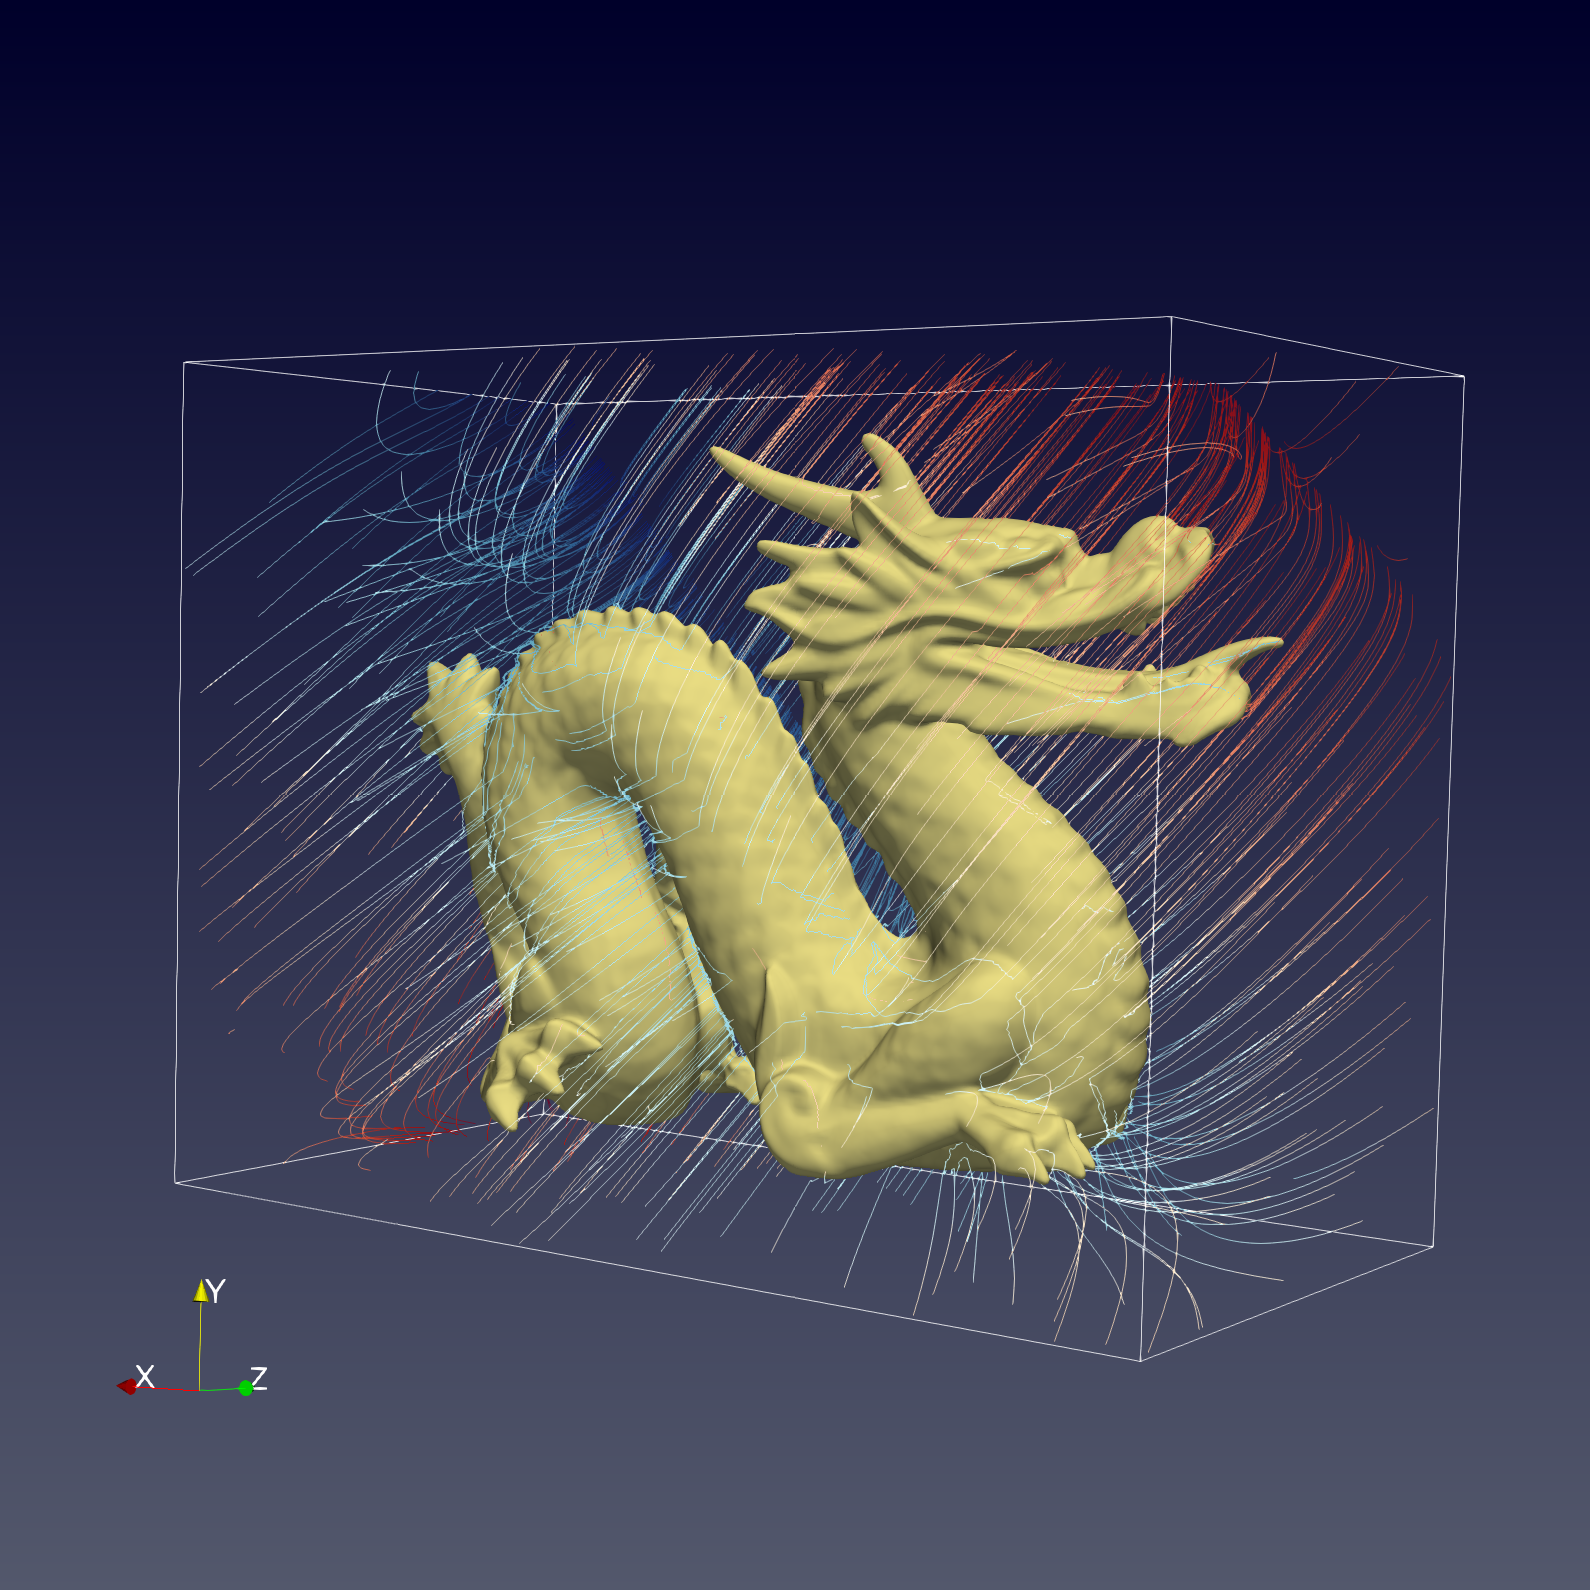
\includegraphics[height=0.32\linewidth]{figures/dragon_streams.png} 
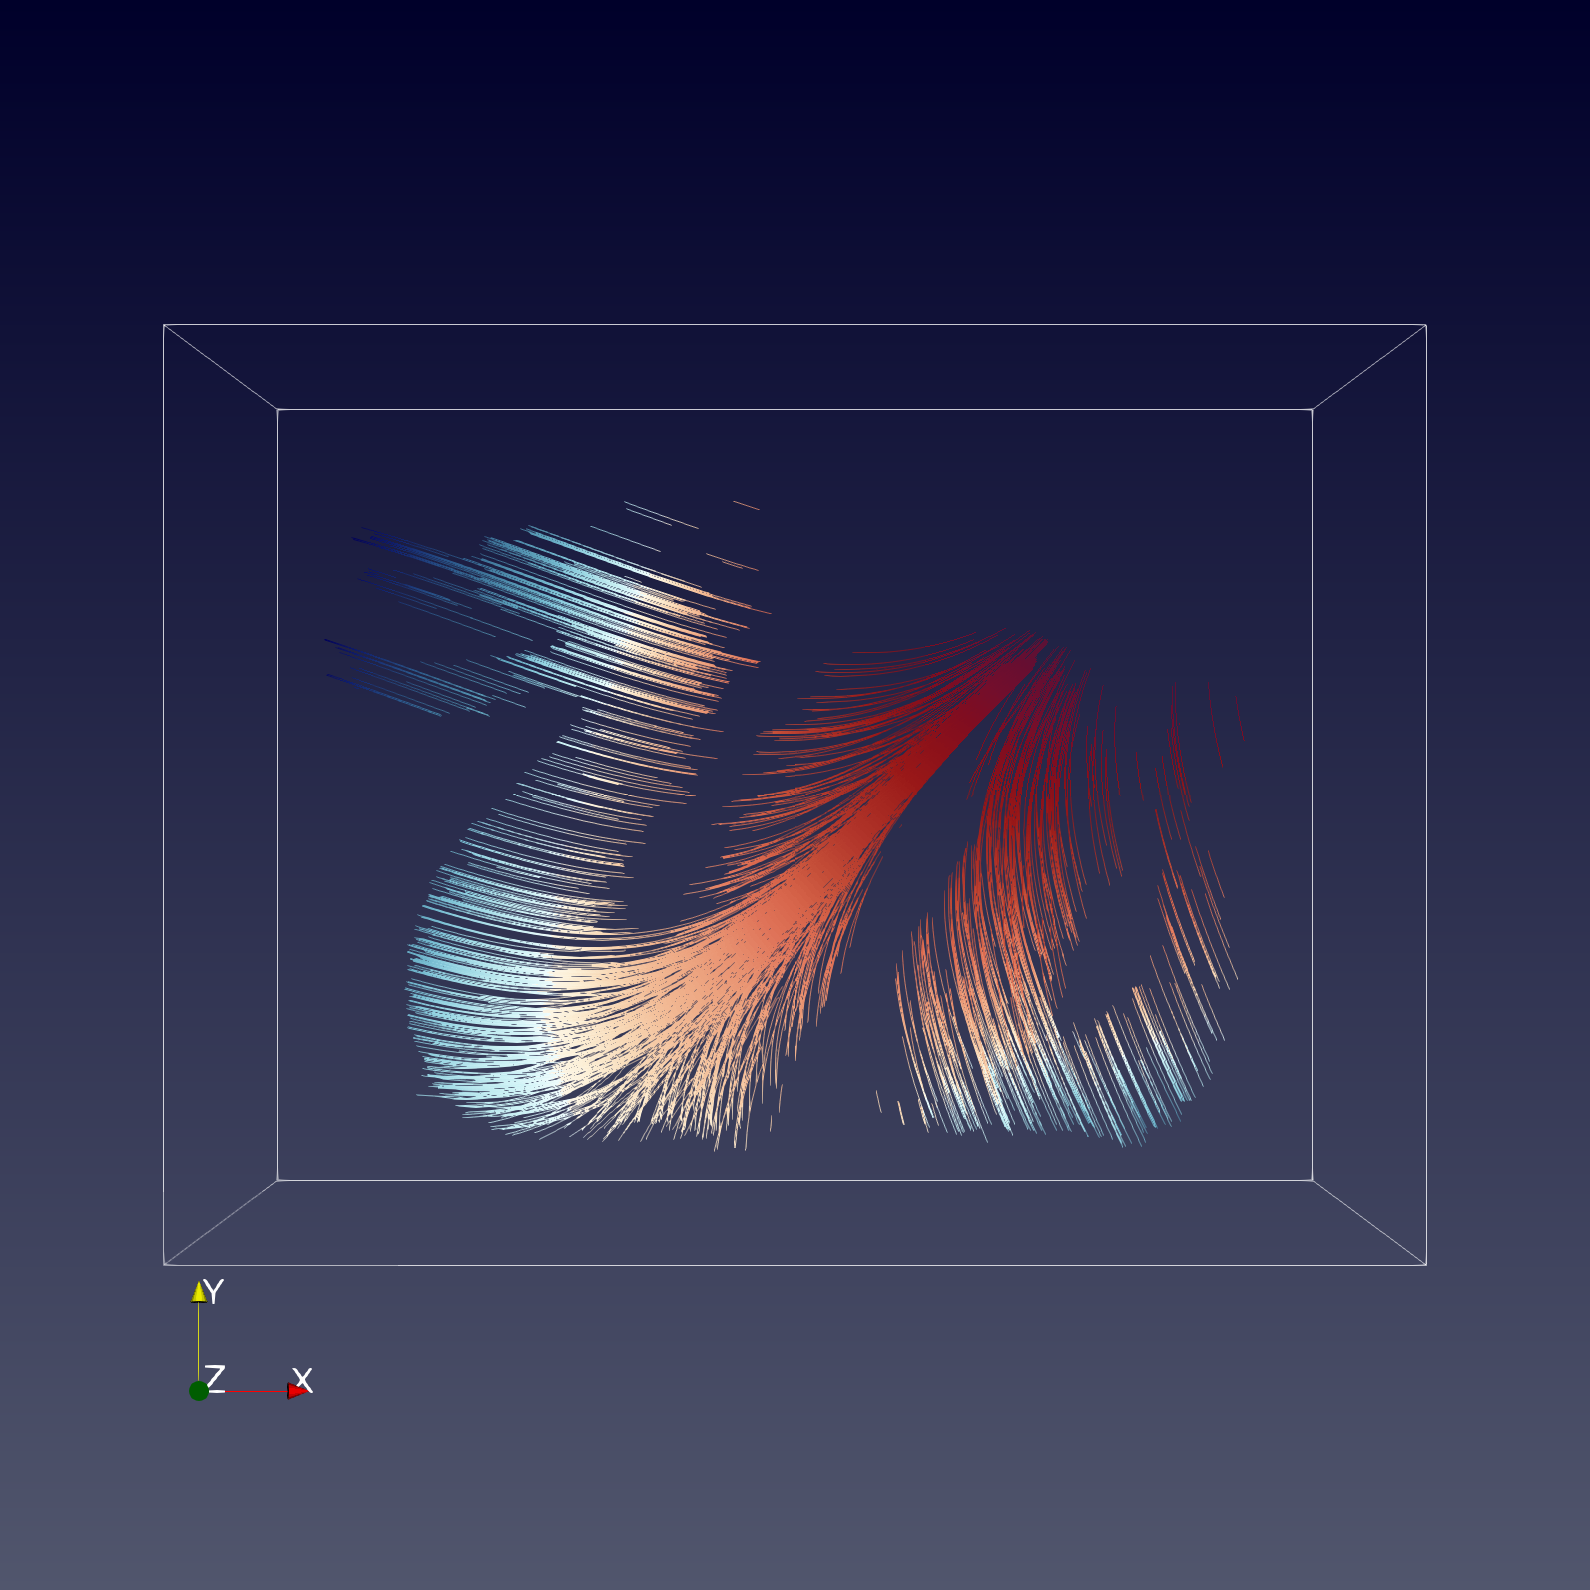
\includegraphics[width=0.32\linewidth]{figures/dragon_streams_inside.png} 
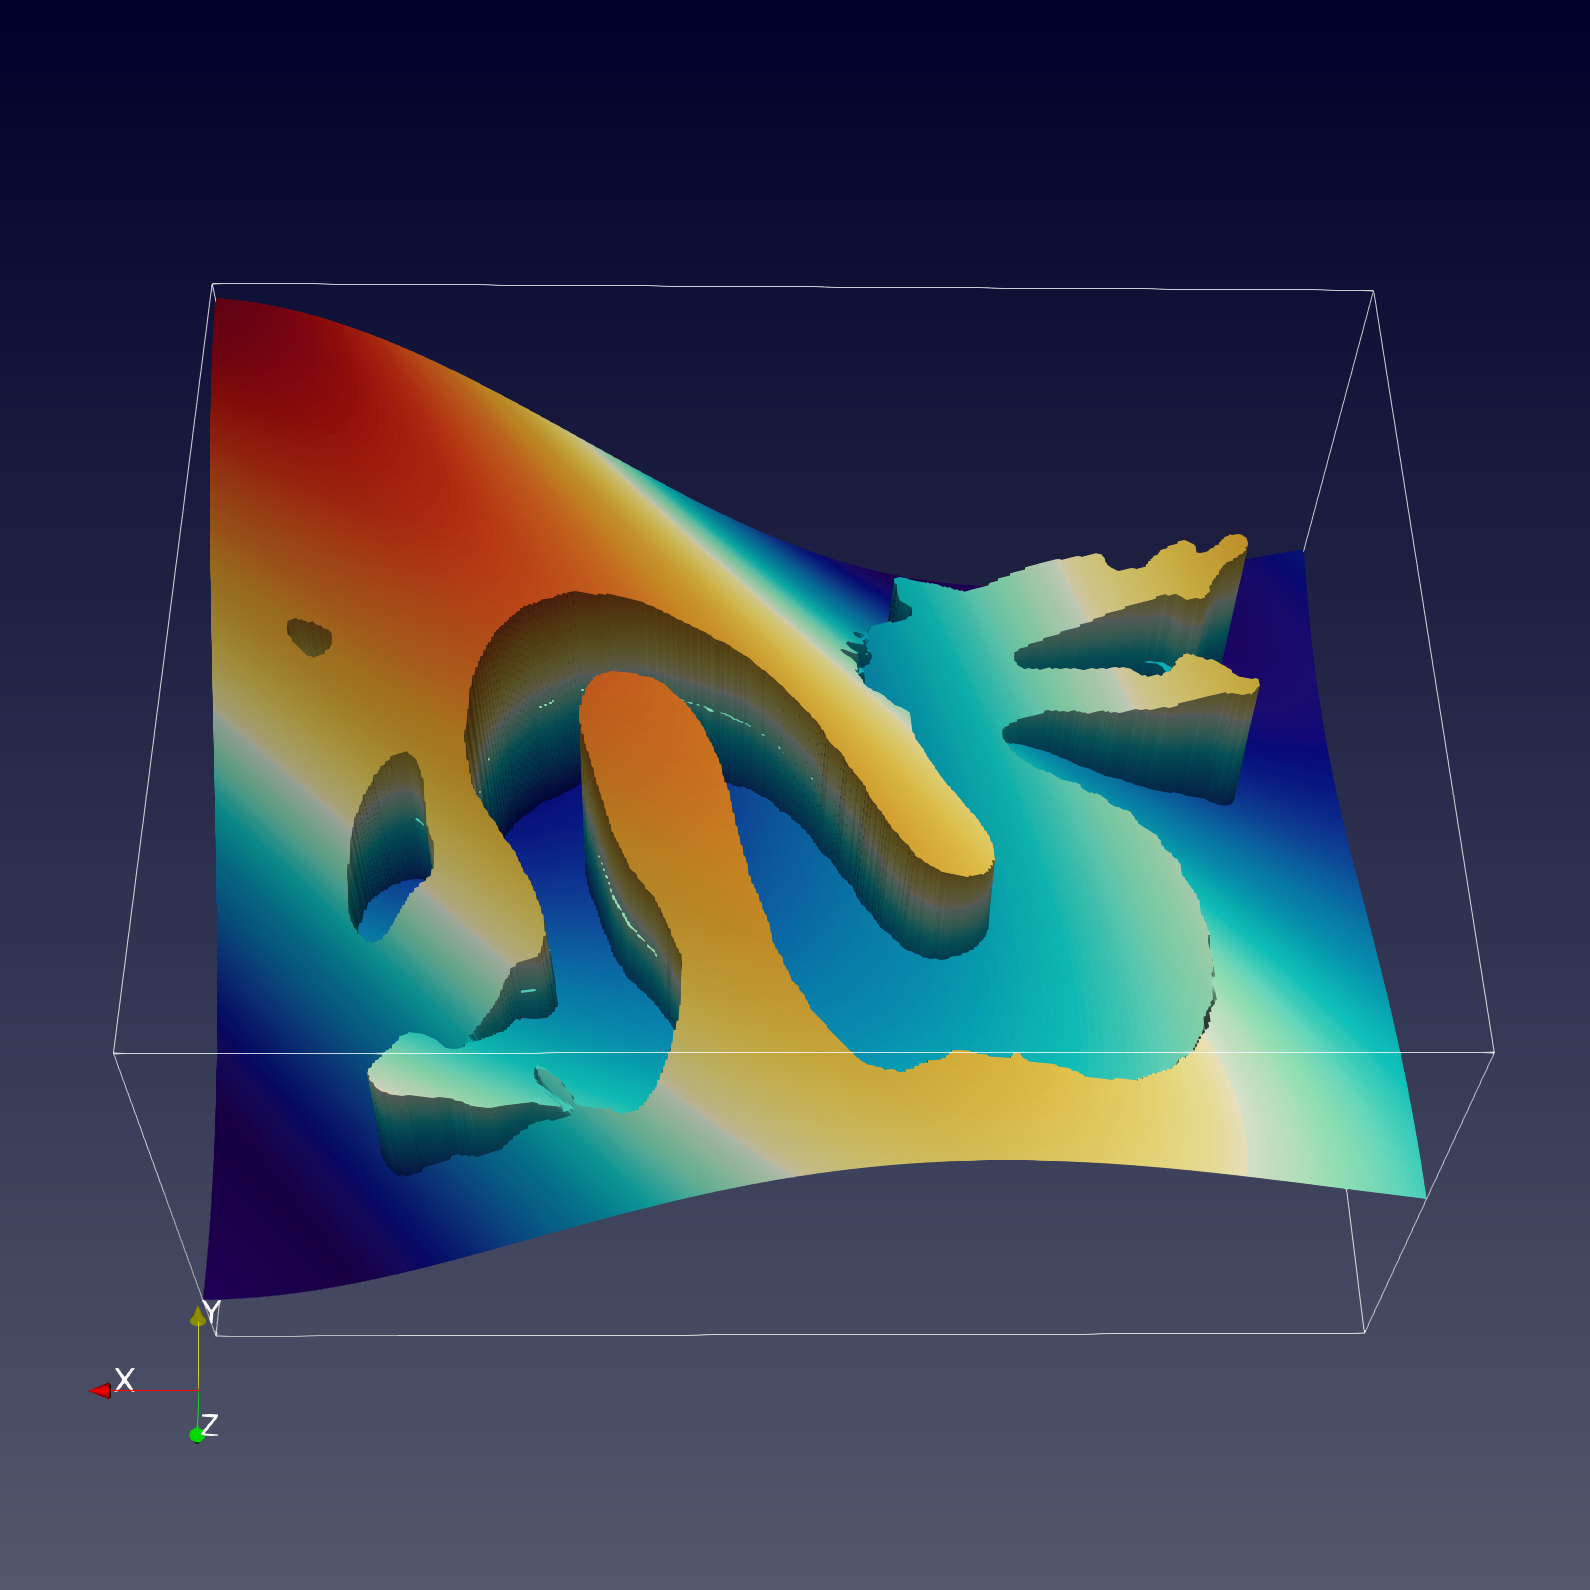
\includegraphics[height=0.32\linewidth]{figures/jump_dragon.png
}
\caption{The proposed Neural Bootstrapping Method applied to computing the electrostatic field around a complex charged geometry in a complex dielectric. The neural approach readily enables a $1024^3$ effective resolution on a single NVIDIA A6000 GPU and captures the physically correct discontinuities. Geometry with gradient streamlines (left), interior streamlines (center), warped cross-section showing jump in solution and gradient.}
\label{fig:dragon}
\end{figure}

\begin{abstract}
 
  We present a highly scalable strategy for developing mesh-free hybrid neuro-symbolic partial differential equation (PDE) solvers based on existing mesh-based numerical discretization methods. Particularly, this strategy can be used to efficiently train neural network surrogate models for the solution functions and operators of PDEs while retaining the accuracy and convergence properties of the state-of-the-art numerical solvers. The presented neural bootstrapping method (hereby dubbed NBM) is based on minimizing residuals of discretized PDE system on an array of implicit Cartesian cells at different levels of resolution centered on a set of random collocation points with respect to trainable parameters of the neural network. NBM leverages neural networks to achieve unprecedented resolution and flexibility for solving PDEs that describe complex physical systems.  
\end{abstract}

%\textcolor{blue}{To put somewhere: (1) In our approach, there is no constraint on where to place the "degrees of freedom", which gives an enormous advantage on how to approach problems. (2) compared to other work, the networks are attached to each point instead of an entire grid. (3) solution to elliptic/parabolic problems have infinite speed of propagation, which means that every grid point influences every other points. Traditional numerical methods capture that property by solving linear systems by iteration. Here this is done during the training by a shared surrogate neural network model.}

%\textcolor{blue}{TODO: We should cite the relevant literature from this conference venue.}

\section{Introduction}
Most modern physical and engineering systems are described by partial differential equations on irregular, often moving, boundaries. The difficulties in solving those problems stem from how to approximate the equations, while respecting the physically correct discontinuous nature of the solution across the boundaries. Smoothing strategies are easy to design, but unfortunately introduce unphysical characteristics in the solution and lead to systemic errors.

Since early 1990s, artificial neural networks have been used for solving partial differential equations by (i) mapping the algebraic operations of the discretized PDE systems onto specialized neural network architectures and minimizing the network energy, or (ii) treating the whole neural network as the basic approximation unit whose parameters are adjusted to minimize a specialized error function that includes the differential equation itself with its boundary/initial conditions. 

In the first category, neurons output the discretized solution values over a set number of grid points and minimizing the network energy drives the neuronal values towards the solution of the linear system at the mesh points. In this case, the neural network energy is the residual of the finite discretization method summed over all neurons of the network \cite{lee1990neural}. Although the convergence properties of the finite discretization methods guarantee and control quality of the obtained solutions, the computational costs grow by increasing resolution and dimensionality. Some early examples include \cite{gobovic1993design,chua1988cellular,chua1988cellularA}.


The second strategy proposed by Lagaris \textit{et al.} \cite{lagaris1998artificial} relies on the function approximation capabilities of the neural networks. Encoding the solution everywhere in the domain within a neural network offers a mesh-free, compact, and memory efficient surrogate model for the solution function that can be utilized in subsequent inference tasks. This method has recently re-emerged as the physics-informed neural networks (PINNs) \cite{RAISSI2019686} and is widely used. Despite their advantages, these methods lack controllable accuracy and convergence properties of finite discretization methods, and are biased towards lower frequency features of the solutions \cite{wang2022and,rahaman2019spectral}.

\textit{Pursuit of hybrid solvers aims at leveraging the performance gains of neural network inference on modern accelerated hardware with the guaranteed accuracy of finite discretization methods. The hybridization efforts are algorithmic or architectural.}

One important algorithmic method is the deep Galerkin method (DGM) \cite{SIRIGNANO20181339} that is a neural network extension of the mesh-free Galerkin method where the solution is represented as a deep neural network rather than a linear combination of basis functions. The mesh-free nature of DGM, that stems from the underlying mesh-free Galerkin method, enables solving problems in higher dimensions by training the neural network model to satisfy the PDE operator and its initial and boundary conditions on a randomly sampled set of points rather than on an exponentially large grid. Although the number of points is huge in higher dimensions, the algorithm can process training on smaller batches of data points sequentially. Besides, second order derivatives in PDEs are calculated by a Monte Carlo method that retain scaling to higher dimensions. Another important algorithmic method is the deep Ritz method for solving variational problems \cite{yu2018deep} that implements a deep nerual network approximation of the trial function that is constrained by numerical quadrature rule for the variational functional, followed by stochastic gradient descent.

Architectural hybridization methods are based on differentiable numerical linear algebra. One emerging class involves implementing differentiable finite discretization solvers and embedding them in the neural network architectures that enable application of end-to-end differentiable gradient based optimization methods. Recently, differentiable solvers have been developed in JAX \cite{jax2018github} for fluid dynamic problems, such as \texttt{Phi-Flow} \cite{holl2020phiflow}, \texttt{JAX-CFD} \cite{Kochkov2021-ML-CFD}, and \texttt{JAX-FLUIDS} \cite{bezgin2022jax}. These methods are suitable for inverse problems where an unknown field is modeled by the neural network, while the model influence is propagated by the differentiable solver into a measurable residual \cite{pakravan2021solving,dal2020data,lu2020extracting}. We also note the classic strategy for solving inverse problems is the adjoint method to obtain the gradient of the loss without differentiation across the solver \cite{berg2017neural}; however, deriving analytic expression for the adjoint equations is tedious, should be repeated after modification of the problem or its loss function, and can become impractical for multiphysics problems. Other important utilities of differentiable solvers are to model and correct for the solution errors of finite discretization methods \cite{um2020solver}, learning and controling PDE systems \cite{de2018end,holl2020learning}.

Neural networks are not only universal approximators of continuous functions, but also of nonlinear operators \cite{chen1995universal}. Although this fact has been leveraged using data-driven strategies for learning differential operators by many authors \cite{lu2019deeponet,bhattacharya2020model,li2020neural,li2020fourier}, current authors have demonstrated utility of differentiable solvers to effectively train nonlinear operators without any data in a completely physics-driven fashion, see section on learning the inverse transforms in \cite{pakravan2021solving}.

In this work we propose a novel framework for solving PDEs based on deep neural networks by lifting any existing mesh-based finite discretization method off of its underlying grid and extend it into a mesh-free method that can be applied to high dimensional problems on unstructured random points in an embarrasingly parallel fashion. In addition, discontinuous solutions can be readily considered.

\section{Problem statement}
In order to illustrate our approach, we consider a closed irregular interface ($\rm \Gamma$) that partitions the computational domain ($\rm \Omega$) into interior ($\rm \Omega^-$) and exterior ($\rm \Omega^+$) subdomains; \textit{i.e.}, $\rm \Omega=\Omega^- \cup \Gamma \cup \Omega^+$. We are interested in the solutions $\rm u^\pm\in \Omega^\pm$ to the following class of linear elliptic problems in  $\rm \mathbf{x}\in\Omega^\pm$:
\begin{align*}
	 & k^{\pm}u^{\pm} - \nabla \cdot (\mu^{\pm}\nabla u^\pm)=f^{\pm}, & \mathbf{x}\in\Omega^\pm \\
	 & [u]=\alpha,                                                    & \mathbf{x} \in \Gamma   \\
	 & [\mu \partial_{\mathbf{n}}u]=\beta,                            & \mathbf{x} \in \Gamma
\end{align*}
Here $f^\pm=f(\mathbf{x} \in \Omega^\pm)$, $\rm \mu^\pm=\mu(\mathbf{x} \in \Omega^\pm)$ and $k^\pm$ are the spatially varying source term, diffusion coefficients, and coefficients, respectively in the two domains. For simplicity, we consider Dirichlet boundary conditions at the boundary of a cubic domain $\rm \Omega=[-L/2,L/2]^3$, noting that other boundary conditions can be readily considered.


This class of problems not only captures the difficulties of solving partial differential equations on irregular domain with discontinuous solutions, but also illustrate their multiscale nature that requires a nonuniform sampling in space. In addition, this system of equations is important on its own as it arises ubiquitously in describing diffusion dominated processes in physical systems and in the life sciences, where sharp and irregular interfaces regulate transport across regions with different properties. Examples include Poisson-Boltzmann equation for describing electrostatic properties of membranes, colloids and solvated biomolecules with jump in dielectric permitivities \cite{sharp1990calculating,MirzadehPB}, in electroporation of cell aggregates with nonlinear membrane jump conditions \cite{mistani2019parallel}, or epitaxial growth in fabrication of opto-electronic devices \cite{MISTANI2018150}. Other important applications are found in solidification of multicomponent alloys \citep{theillard2015sharp,bochkov2021sharp}, directed self-assembly of diblock copolymers for next generation lithography \cite{galatsis2010patterning,ouaknin2018level,bochkov2021non}, multiphase flows with and without phase change. 





\section{Scalable \& Mesh-Freeing Neuro-Symbolic PDE Solver}



\begin{figure}
\centering
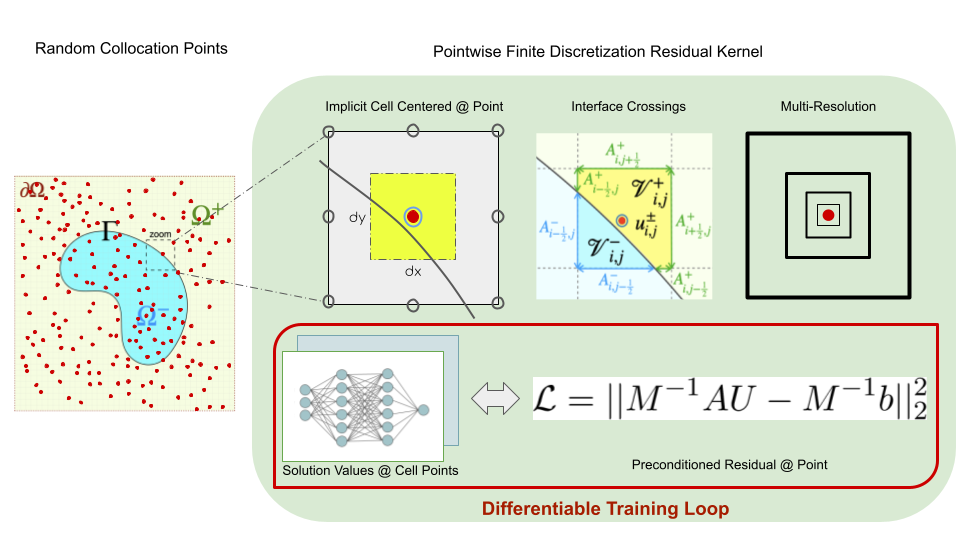
\includegraphics[width=0.85\textwidth]{./figures/jax_dips_paper_v1_compact.png}
\caption{Neural Bootstrapping Method (NBM). NBM kernels compute residual contribution by each collocation point per GPU thread. Kernel operations involve implicit cells at different resolutions according to the bootstrapped finite discretization method. Geometric information for interface-cell crossings is computed by a level-set interpolant defined on a much lower resolution grid. Pointwise residuals are locally preconditioned based on the geometry of the interface crossing the implicit cells. }
\label{fig:nbm}
\end{figure}
Neural networks are used as surrogates for the solution function that are iteratively adjusted to minimize discretization residuals at a set of randomly sampled points and at arbitrary resolutions. The key idea is that neural networks can be evaluated over vertices of any discretization stencils centered at any point in the domain effectively emulating the effect of any structured mesh without ever materializing the mesh. Therefore, we use neural networks to bootstrap mesh based finite discretization (FD) methods to compile mesh free numerical methods. We call this the Neural Bootstrapping Method (NBM), and illustrate it in figure \ref{fig:nbm}. 

FD methods offer guaranteed accuracy and controllable convergence properties for the training of neural network surrogate models of physical systems. NBM offers a straightforward path for applying mesh-based FD methods on unstructured random points. This is an important ability for augmenting observational data in the training pipelines. Beside its mesh-freeing advantage, NBM is a highly parallelizable strategy for FD methods. Pointwise nature of its kernels is ideally suited for GPU-accelerated computing paradigm. Multi-GPU parallel solution of PDE systems is reduced to the much simpler problem of data-parallel training using existing machine learning frameworks. Data parallelism involves distributing collocation points across multiple processors to compute gradient updates and then aggregating these locally computed updates \cite{shallue2018measuring}.

Here we bootstrap the numerical scheme proposed by \cite{BOCHKOV2020109269}, hence the loss function is 
\begin{align*}
\mathcal{L} = & \bigg\vert\bigg\vert \sum_{s=-,+} k_{i,j}^s u_{i,j}^{s} |\mathcal{V}_{i,j}^s| - \sum_{s=-,+}\bigg( \mu_{i-\frac{1}{2},j}^s A_{i-\frac{1}{2},j}^s\frac{u_{i-1,j}^s - u_{i,j}^s}{\Delta x}     +   \mu_{i+\frac{1}{2},j}^s A_{i+\frac{1}{2},j}^s\frac{u_{i+1,j}^s - u_{i,j}^s}{\Delta x} +                                                          \\
	 & \mu_{i, j-\frac{1}{2}}^s A_{i, j-\frac{1}{2}}^s\frac{u_{i,j-1}^s - u_{i,j}^s}{\Delta y} + \mu_{i, j+\frac{1}{2}}^s A_{i, j+\frac{1}{2}}^s\frac{u_{i,j+1}^s - u_{i,j}^s}{\Delta y} \bigg)  -  \sum_{s=-,+} f_{i,j}^{s} |\mathcal{V}_{i,j}^s| - \int_{\Gamma\cap \mathcal{V}_{i,j}} \beta d\Gamma \bigg\vert\bigg\vert_2^2
\end{align*}
Operations in differentiable NBM kernels are strictly local. NBM starts by placing implicit compute cells of a specified resolutions at the collocation point. At the presence of discontinuities a separate coarse mesh encapsulates an interpolant for the level-set function whose intersection with the NBM cell is calculated to obtain geometric information for the FD kernel and preconditioner (denoted $M^{-1}$). FD kernel is applied on the compute cell where the solution values are evaluated by the neural network. Each kernel contributes a local $L^2$-norm residual $r_p = ||M^{-1}A U - M^{-1}b||$ at one point $p$. Preconditioning helps to balance relative magnitude of contributions from all points before aggregating residuals to form a global loss value. Finally, gradient based optimization methods used in machine learning are applied to adjust neural network parameters. The automatic differentiation loop passes across the NBM kernels.








\section{Numerical results}
\subsection{Convergence}

We consider a sphere centered at the origin with radius 1/2 in a domain $[0, 1]^3$, an exact solution $u^-(x,y,z)=e^{z}$ inside and $u^+(x,y,z)=\cos(x)\sin(y)$ outside. In addition to the jump in solution, we also consider a jump in the variable diffusion coefficient to be $\mu^-(x,y,z)=y^2 \ln(x+2) + 4$ inside and $\mu^+(x,y,z)=e^{-z}$ outside the sphere. Table \ref{tab:convergence} reports convergence results for the solution, which illustrates the convergence in the $L^\infty$-norm. Two neural networks were used to represent solutions inside and outside the sphere with 5 hidden layers and 10 sine-activated neurons each.


\begin{table}[ht]
\begin{center}
\caption{We report $L^\infty$-norm error and root-mean-squared-error (RMSE) of the solution field evaluated in the domain. Rightmost column reports the overall time to solution for our JAX implementation which constitutes $10,000$ epochs in each case and the initial compilation time of jaxpressions. A pair of neural networks, each with 5 hidden layers of 10 neurons wide, have $982$ total trainable parameters. In each case GPU compute occupancy is at $100\%$ on a single NVIDIA RTX A6000 GPU. } \label{tab:convergence}

\begin{tabular}{|l||ll|ll|c|c|}
\hline
regress $\partial_n$ & \multicolumn{2}{c|}{RMSE}& \multicolumn{2}{c|}{$L^\infty$} & \multicolumn{2}{c|}{GPU Statistics} \\
\hline
$\rm N_{x,y,z}$   &   Solution    &   Order   &   Solution   &   Order & t (sec/epoch) & VRAM (GB)\\
\hline 
$2^3$ & $3.7\times 10^{-2}$ &  -        & $3.25\times 10^{-1}$  &   -     & $0.0306$ & $1.05$ \\
$2^4$ & $7.1\times 10^{-3}$ &  $2.38$   & $1.10\times 10^{-1}$   & $1.56$  & $0.056$  & $1.72$ \\ 
$2^5$ & $5.9\times 10^{-3}$ &  $0.27$   & $8.36 \times 10^{-2}$ & $0.4$   & $0.053$  & $2.15$ \\ 
$2^6$ & $4.1\times 10^{-3}$ &  $0.53$   & $6.44\times 10^{-2}$  & $0.38$  & $0.287$  & $5.57$ \\ 
$2^7$ & $2.64\times 10^{-3}$&  $0.64$   & $3.53\times 10^{-2}$  & $0.87$  & $2.125$ & $32.1$ \\ \hline
\end{tabular}
\end{center}
\end{table}

\subsection{Complex geometry and physics}
We simulate a Poisson problem with discontinuities on the Dragon problem presented in \cite{curless1996volumetric}. In this case we used the signed-distance function produced by SDFGen, and initiated an interpolant based on its values. An exact solution $u^-(x,y,z)=\sin(2x)\cos(2y) e^{z}$ inside and
$u^+(x,y,z)=\bigg[ 16\big(\frac{y-x}{3}\big)^5 - 20 \big(\frac{y-x}{3}\big)^3 + 5\big( \frac{y-x}{3}\big) \bigg]\ln(x+y+3)\cos(z)$ outside with variable diffusion coefficients $\mu^-(x,y,z)=10\bigg[ 1+0.2\cos(2\pi(x+y))\sin(2\pi(x-y)) \cos(z) \bigg] $ inside and $\mu^+(x,y,z)=1$ outside. The results are shown in figure \ref{fig:dragon}, with $\rm L^\infty$-norm of $0.5$ and RMSE of $0.06$ after 1000 epochs on multi-resolutions $64^3,128^3,256^3,512^3$. The neural network pair have only 1 hidden layer with 100 sine-activated neurons.



\subsection{Time complexity and parallel scaling on GPU clusters}
In table \ref{tab:scaling} we report timings at different resolutions distributed across different number of NVIDIA A100 GPUs. We used a batchsize of $32\times 32\times 16$ in all cases. At fixed number of GPUs, training time scales linearly with number of grid points, $\mathcal{O}(N)$. At a fixed resolution, increasing number of GPUs consistently decreases training time roughly with $\rm epoch\ time \sim 1/\sqrt{GPU\ count}$, although the advantage is more effective at higher resolutions. Compile time for \textit{jaxpressions} increases with resolution and decreases with number of GPUs.

A maximum grid size of $1024^3$ at multi-resolutions $1024^3,\ 2048^3, 4096^3,\ 8192^3$ was simulated on a DGX machine with 8 NVIDIA A100 GPUs taking almost $30$ minutes per epoch. 

\begin{table}[ht]
\begin{center}
\caption{Scaling test. Time per epoch (sec) and JAX compile time for different configurations.} \label{tab:scaling}
\begin{tabular}{|c||cc|cc|cc|cc|}
\hline
base resolution & \multicolumn{2}{c|}{$64^3$}& \multicolumn{2}{c|}{$128^3$} & \multicolumn{2}{c|}{$256^3$}  & \multicolumn{2}{c|}{$512^3$}\\
\hline
$\rm A100\ GPUs$ &  epoch  &  compile   &  epoch   & compile &    epoch & compile  &  epoch    &   compile \\
\hline 
$1$        & $0.908$ &  $9.027$   & $6.960$  & $9.288$ & $55.287$ & $12.164$ &  $438.45$  &  $49.020$ \\
$2$        & $0.657$ &  $7.575$   & $5.893$  & $7.823$ & $47.360$ & $10.045$ &  $378.98$  &  $39.815$ \\ 
$4$        & $0.405$ &  $7.480$   & $3.629$  & $7.863$ & $28.261$ & $9.129$  &  $226.73$  &  $27.405$ \\ 
$8$        & $0.384$ &  $7.983$   & $3.340$  & $7.901$ & $26.799$ & $9.154$  &  $204.88$  &  $20.632$\\ \hline
\end{tabular}
\end{center}
\end{table}


\section{Conclusion}
We presented neural bootstrapping method and applied it to the problem of solving elliptic PDEs with discontinuities. We implemented the method using JAX and showed accuracy and parallel scaling on test problems. NBM is a differentiable computing method that makes mesh-free numerical methods based on mesh-based finite discretization methods by representing the solutions by training neural networks using automatic differentiation of the discretized residual over a set of collocation points.




\newpage
\color{red}
The following describes the formatting of a NeurIPS paper:
\section{Submission of papers to NeurIPS 2022}


Please read the instructions below carefully and follow them faithfully.


\subsection{Style}


Papers to be submitted to NeurIPS 2022 must be prepared according to the
instructions presented here. Papers may only be up to {\bf nine} pages long,
including figures. Additional pages \emph{containing only acknowledgments and
references} are allowed. Papers that exceed the page limit will not be
reviewed, or in any other way considered for presentation at the conference.


The margins in 2022 are the same as those in 2007, which allow for $\sim$$15\%$
more words in the paper compared to earlier years.


Authors are required to use the NeurIPS \LaTeX{} style files obtainable at the
NeurIPS website as indicated below. Please make sure you use the current files
and not previous versions. Tweaking the style files may be grounds for
rejection.


\subsection{Retrieval of style files}


The style files for NeurIPS and other conference information are available on
the World Wide Web at
\begin{center}
  \url{http://www.neurips.cc/}
\end{center}
The file \verb+neurips_2022.pdf+ contains these instructions and illustrates the
various formatting requirements your NeurIPS paper must satisfy.


The only supported style file for NeurIPS 2022 is \verb+neurips_2022.sty+,
rewritten for \LaTeXe{}.  \textbf{Previous style files for \LaTeX{} 2.09,
  Microsoft Word, and RTF are no longer supported!}


The \LaTeX{} style file contains three optional arguments: \verb+final+, which
creates a camera-ready copy, \verb+preprint+, which creates a preprint for
submission to, e.g., arXiv, and \verb+nonatbib+, which will not load the
\verb+natbib+ package for you in case of package clash.


\paragraph{Preprint option}
If you wish to post a preprint of your work online, e.g., on arXiv, using the
NeurIPS style, please use the \verb+preprint+ option. This will create a
nonanonymized version of your work with the text ``Preprint. Work in progress.''
in the footer. This version may be distributed as you see fit. Please \textbf{do
  not} use the \verb+final+ option, which should \textbf{only} be used for
papers accepted to NeurIPS.


At submission time, please omit the \verb+final+ and \verb+preprint+
options. This will anonymize your submission and add line numbers to aid
review. Please do \emph{not} refer to these line numbers in your paper as they
will be removed during generation of camera-ready copies.


The file \verb+neurips_2022.tex+ may be used as a ``shell'' for writing your
paper. All you have to do is replace the author, title, abstract, and text of
the paper with your own.


The formatting instructions contained in these style files are summarized in
Sections \ref{gen_inst}, \ref{headings}, and \ref{others} below.


\section{General formatting instructions}
\label{gen_inst}


The text must be confined within a rectangle 5.5~inches (33~picas) wide and
9~inches (54~picas) long. The left margin is 1.5~inch (9~picas).  Use 10~point
type with a vertical spacing (leading) of 11~points.  Times New Roman is the
preferred typeface throughout, and will be selected for you by default.
Paragraphs are separated by \nicefrac{1}{2}~line space (5.5 points), with no
indentation.


The paper title should be 17~point, initial caps/lower case, bold, centered
between two horizontal rules. The top rule should be 4~points thick and the
bottom rule should be 1~point thick. Allow \nicefrac{1}{4}~inch space above and
below the title to rules. All pages should start at 1~inch (6~picas) from the
top of the page.


For the final version, authors' names are set in boldface, and each name is
centered above the corresponding address. The lead author's name is to be listed
first (left-most), and the co-authors' names (if different address) are set to
follow. If there is only one co-author, list both author and co-author side by
side.


Please pay special attention to the instructions in Section \ref{others}
regarding figures, tables, acknowledgments, and references.


\section{Headings: first level}
\label{headings}


All headings should be lower case (except for first word and proper nouns),
flush left, and bold.


First-level headings should be in 12-point type.


\subsection{Headings: second level}


Second-level headings should be in 10-point type.


\subsubsection{Headings: third level}


Third-level headings should be in 10-point type.


\paragraph{Paragraphs}


There is also a \verb+\paragraph+ command available, which sets the heading in
bold, flush left, and inline with the text, with the heading followed by 1\,em
of space.


\section{Citations, figures, tables, references}
\label{others}


These instructions apply to everyone.


\subsection{Citations within the text}


The \verb+natbib+ package will be loaded for you by default.  Citations may be
author/year or numeric, as long as you maintain internal consistency.  As to the
format of the references themselves, any style is acceptable as long as it is
used consistently.


The documentation for \verb+natbib+ may be found at
\begin{center}
  \url{http://mirrors.ctan.org/macros/latex/contrib/natbib/natnotes.pdf}
\end{center}
Of note is the command \verb+\citet+, which produces citations appropriate for
use in inline text.  For example,
\begin{verbatim}
   \citet{hasselmo} investigated\dots
\end{verbatim}
produces
\begin{quote}
  Hasselmo, et al.\ (1995) investigated\dots
\end{quote}


If you wish to load the \verb+natbib+ package with options, you may add the
following before loading the \verb+neurips_2022+ package:
\begin{verbatim}
   \PassOptionsToPackage{options}{natbib}
\end{verbatim}


If \verb+natbib+ clashes with another package you load, you can add the optional
argument \verb+nonatbib+ when loading the style file:
\begin{verbatim}
   \usepackage[nonatbib]{neurips_2022}
\end{verbatim}


As submission is double blind, refer to your own published work in the third
person. That is, use ``In the previous work of Jones et al.\ [4],'' not ``In our
previous work [4].'' If you cite your other papers that are not widely available
(e.g., a journal paper under review), use anonymous author names in the
citation, e.g., an author of the form ``A.\ Anonymous.''


\subsection{Footnotes}


Footnotes should be used sparingly.  If you do require a footnote, indicate
footnotes with a number\footnote{Sample of the first footnote.} in the
text. Place the footnotes at the bottom of the page on which they appear.
Precede the footnote with a horizontal rule of 2~inches (12~picas).


Note that footnotes are properly typeset \emph{after} punctuation
marks.\footnote{As in this example.}


\subsection{Figures}


\begin{figure}
  \centering
  \fbox{\rule[-.5cm]{0cm}{4cm} \rule[-.5cm]{4cm}{0cm}}
  \caption{Sample figure caption.}
\end{figure}


All artwork must be neat, clean, and legible. Lines should be dark enough for
purposes of reproduction. The figure number and caption always appear after the
figure. Place one line space before the figure caption and one line space after
the figure. The figure caption should be lower case (except for first word and
proper nouns); figures are numbered consecutively.


You may use color figures.  However, it is best for the figure captions and the
paper body to be legible if the paper is printed in either black/white or in
color.


\subsection{Tables}


All tables must be centered, neat, clean and legible.  The table number and
title always appear before the table.  See Table~\ref{sample-table}.


Place one line space before the table title, one line space after the
table title, and one line space after the table. The table title must
be lower case (except for first word and proper nouns); tables are
numbered consecutively.


Note that publication-quality tables \emph{do not contain vertical rules.} We
strongly suggest the use of the \verb+booktabs+ package, which allows for
typesetting high-quality, professional tables:
\begin{center}
  \url{https://www.ctan.org/pkg/booktabs}
\end{center}
This package was used to typeset Table~\ref{sample-table}.


\begin{table}
  \caption{Sample table title}
  \label{sample-table}
  \centering
  \begin{tabular}{lll}
    \toprule
    \multicolumn{2}{c}{Part}                   \\
    \cmidrule(r){1-2}
    Name     & Description     & Size ($\mu$m) \\
    \midrule
    Dendrite & Input terminal  & $\sim$100     \\
    Axon     & Output terminal & $\sim$10      \\
    Soma     & Cell body       & up to $10^6$  \\
    \bottomrule
  \end{tabular}
\end{table}


\section{Final instructions}


Do not change any aspects of the formatting parameters in the style files.  In
particular, do not modify the width or length of the rectangle the text should
fit into, and do not change font sizes (except perhaps in the
\textbf{References} section; see below). Please note that pages should be
numbered.


\section{Preparing PDF files}


Please prepare submission files with paper size ``US Letter,'' and not, for
example, ``A4.''


Fonts were the main cause of problems in the past years. Your PDF file must only
contain Type 1 or Embedded TrueType fonts. Here are a few instructions to
achieve this.


\begin{itemize}


\item You should directly generate PDF files using \verb+pdflatex+.


\item You can check which fonts a PDF files uses.  In Acrobat Reader, select the
  menu Files$>$Document Properties$>$Fonts and select Show All Fonts. You can
  also use the program \verb+pdffonts+ which comes with \verb+xpdf+ and is
  available out-of-the-box on most Linux machines.


\item The IEEE has recommendations for generating PDF files whose fonts are also
  acceptable for NeurIPS. Please see
  \url{http://www.emfield.org/icuwb2010/downloads/IEEE-PDF-SpecV32.pdf}


\item \verb+xfig+ "patterned" shapes are implemented with bitmap fonts.  Use
  "solid" shapes instead.


\item The \verb+\bbold+ package almost always uses bitmap fonts.  You should use
  the equivalent AMS Fonts:
\begin{verbatim}
   \usepackage{amsfonts}
\end{verbatim}
followed by, e.g., \verb+\mathbb{R}+, \verb+\mathbb{N}+, or \verb+\mathbb{C}+
for $\mathbb{R}$, $\mathbb{N}$ or $\mathbb{C}$.  You can also use the following
workaround for reals, natural and complex:
\begin{verbatim}
   \newcommand{\RR}{I\!\!R} %real numbers
   \newcommand{\Nat}{I\!\!N} %natural numbers
   \newcommand{\CC}{I\!\!\!\!C} %complex numbers
\end{verbatim}
Note that \verb+amsfonts+ is automatically loaded by the \verb+amssymb+ package.


\end{itemize}


If your file contains type 3 fonts or non embedded TrueType fonts, we will ask
you to fix it.


\subsection{Margins in \LaTeX{}}


Most of the margin problems come from figures positioned by hand using
\verb+\special+ or other commands. We suggest using the command
\verb+\includegraphics+ from the \verb+graphicx+ package. Always specify the
figure width as a multiple of the line width as in the example below:
\begin{verbatim}
   \usepackage[pdftex]{graphicx} ...
   \includegraphics[width=0.8\linewidth]{myfile.pdf}
\end{verbatim}
See Section 4.4 in the graphics bundle documentation
(\url{http://mirrors.ctan.org/macros/latex/required/graphics/grfguide.pdf})


A number of width problems arise when \LaTeX{} cannot properly hyphenate a
line. Please give LaTeX hyphenation hints using the \verb+\-+ command when
necessary.


\begin{ack}
Use unnumbered first level headings for the acknowledgments. All acknowledgments
go at the end of the paper before the list of references. Moreover, you are required to declare
funding (financial activities supporting the submitted work) and competing interests (related financial activities outside the submitted work).
More information about this disclosure can be found at: \url{https://neurips.cc/Conferences/2022/PaperInformation/FundingDisclosure}.


Do {\bf not} include this section in the anonymized submission, only in the final paper. You can use the \texttt{ack} environment provided in the style file to autmoatically hide this section in the anonymized submission.
\end{ack}


\section*{References}


References follow the acknowledgments. Use unnumbered first-level heading for
the references. Any choice of citation style is acceptable as long as you are
consistent. It is permissible to reduce the font size to \verb+small+ (9 point)
when listing the references.
Note that the Reference section does not count towards the page limit.
\medskip


{
\small


[1] Alexander, J.A.\ \& Mozer, M.C.\ (1995) Template-based algorithms for
connectionist rule extraction. In G.\ Tesauro, D.S.\ Touretzky and T.K.\ Leen
(eds.), {\it Advances in Neural Information Processing Systems 7},
pp.\ 609--616. Cambridge, MA: MIT Press.


[2] Bower, J.M.\ \& Beeman, D.\ (1995) {\it The Book of GENESIS: Exploring
  Realistic Neural Models with the GEneral NEural SImulation System.}  New York:
TELOS/Springer--Verlag.


[3] Hasselmo, M.E., Schnell, E.\ \& Barkai, E.\ (1995) Dynamics of learning and
recall at excitatory recurrent synapses and cholinergic modulation in rat
hippocampal region CA3. {\it Journal of Neuroscience} {\bf 15}(7):5249-5262.
}


%%%%%%%%%%%%%%%%%%%%%%%%%%%%%%%%%%%%%%%%%%%%%%%%%%%%%%%%%%%%
\section*{Checklist}


%%% BEGIN INSTRUCTIONS %%%
The checklist follows the references.  Please
read the checklist guidelines carefully for information on how to answer these
questions.  For each question, change the default \answerTODO{} to \answerYes{},
\answerNo{}, or \answerNA{}.  You are strongly encouraged to include a {\bf
justification to your answer}, either by referencing the appropriate section of
your paper or providing a brief inline description.  For example:
\begin{itemize}
  \item Did you include the license to the code and datasets? \answerYes{See Section~\ref{gen_inst}.}
  \item Did you include the license to the code and datasets? \answerNo{The code and the data are proprietary.}
  \item Did you include the license to the code and datasets? \answerNA{}
\end{itemize}
Please do not modify the questions and only use the provided macros for your
answers.  Note that the Checklist section does not count towards the page
limit.  In your paper, please delete this instructions block and only keep the
Checklist section heading above along with the questions/answers below.
%%% END INSTRUCTIONS %%%


\begin{enumerate}


\item For all authors...
\begin{enumerate}
  \item Do the main claims made in the abstract and introduction accurately reflect the paper's contributions and scope?
    \answerTODO{}
  \item Did you describe the limitations of your work?
    \answerTODO{}
  \item Did you discuss any potential negative societal impacts of your work?
    \answerTODO{}
  \item Have you read the ethics review guidelines and ensured that your paper conforms to them?
    \answerTODO{}
\end{enumerate}


\item If you are including theoretical results...
\begin{enumerate}
  \item Did you state the full set of assumptions of all theoretical results?
    \answerTODO{}
        \item Did you include complete proofs of all theoretical results?
    \answerTODO{}
\end{enumerate}


\item If you ran experiments...
\begin{enumerate}
  \item Did you include the code, data, and instructions needed to reproduce the main experimental results (either in the supplemental material or as a URL)?
    \answerTODO{}
  \item Did you specify all the training details (e.g., data splits, hyperparameters, how they were chosen)?
    \answerTODO{}
        \item Did you report error bars (e.g., with respect to the random seed after running experiments multiple times)?
    \answerTODO{}
        \item Did you include the total amount of compute and the type of resources used (e.g., type of GPUs, internal cluster, or cloud provider)?
    \answerTODO{}
\end{enumerate}


\item If you are using existing assets (e.g., code, data, models) or curating/releasing new assets...
\begin{enumerate}
  \item If your work uses existing assets, did you cite the creators?
    \answerTODO{}
  \item Did you mention the license of the assets?
    \answerTODO{}
  \item Did you include any new assets either in the supplemental material or as a URL?
    \answerTODO{}
  \item Did you discuss whether and how consent was obtained from people whose data you're using/curating?
    \answerTODO{}
  \item Did you discuss whether the data you are using/curating contains personally identifiable information or offensive content?
    \answerTODO{}
\end{enumerate}


\item If you used crowdsourcing or conducted research with human subjects...
\begin{enumerate}
  \item Did you include the full text of instructions given to participants and screenshots, if applicable?
    \answerTODO{}
  \item Did you describe any potential participant risks, with links to Institutional Review Board (IRB) approvals, if applicable?
    \answerTODO{}
  \item Did you include the estimated hourly wage paid to participants and the total amount spent on participant compensation?
    \answerTODO{}
\end{enumerate}


\end{enumerate}


%%%%%%%%%%%%%%%%%%%%%%%%%%%%%%%%%%%%%%%%%%%%%%%%%%%%%%%%%%%%


\appendix


\section{Appendix}


Optionally include extra information (complete proofs, additional experiments and plots) in the appendix.
This section will often be part of the supplemental material.

%%%%%%%%%%%
\newpage
%\section*{References}
\bibliographystyle{abbrv}
\addcontentsline{toc}{section}{\refname}
\bibliography{references}

\end{document}